% Created 2022-09-20 ti 11:43
% Intended LaTeX compiler: pdflatex
\documentclass[12pt]{article}

%%%% settings when exporting code %%%% 

\usepackage{listings}
\lstdefinestyle{code-small}{
backgroundcolor=\color{white}, % background color for the code block
basicstyle=\ttfamily\small, % font used to display the code
commentstyle=\color[rgb]{0.5,0,0.5}, % color used to display comments in the code
keywordstyle=\color{black}, % color used to highlight certain words in the code
numberstyle=\ttfamily\tiny\color{gray}, % color used to display the line numbers
rulecolor=\color{black}, % color of the frame
stringstyle=\color[rgb]{0,.5,0},  % color used to display strings in the code
breakatwhitespace=false, % sets if automatic breaks should only happen at whitespace
breaklines=true, % sets automatic line breaking
columns=fullflexible,
frame=single, % adds a frame around the code (non,leftline,topline,bottomline,lines,single,shadowbox)
keepspaces=true, % % keeps spaces in text, useful for keeping indentation of code
literate={~}{$\sim$}{1}, % symbol properly display via latex
numbers=none, % where to put the line-numbers; possible values are (none, left, right)
numbersep=10pt, % how far the line-numbers are from the code
showspaces=false,
showstringspaces=false,
stepnumber=1, % the step between two line-numbers. If it's 1, each line will be numbered
tabsize=1,
xleftmargin=0cm,
emph={anova,apply,class,coef,colnames,colNames,colSums,dim,dcast,for,ggplot,head,if,ifelse,is.na,lapply,list.files,library,logLik,melt,plot,require,rowSums,sapply,setcolorder,setkey,str,summary,tapply},
aboveskip = \medskipamount, % define the space above displayed listings.
belowskip = \medskipamount, % define the space above displayed listings.
lineskip = 0pt} % specifies additional space between lines in listings
\lstset{style=code-small}
%%%% packages %%%%%

\usepackage[utf8]{inputenc}
\usepackage[T1]{fontenc}
\usepackage{lmodern}
\usepackage{textcomp}
\usepackage{color}
\usepackage{graphicx}
\usepackage{grffile}
\usepackage{wrapfig}
\usepackage{rotating}
\usepackage{longtable}
\usepackage{multirow}
\usepackage{multicol}
\usepackage{changes}
\usepackage{pdflscape}
\usepackage{geometry}
\usepackage[normalem]{ulem}
\usepackage{amssymb}
\usepackage{amsmath}
\usepackage{amsfonts}
\usepackage{dsfont}
\usepackage{array}
\usepackage{ifthen}
\usepackage{hyperref}
\usepackage{natbib}
\RequirePackage{setspace} % to modify the space between lines - incompatible with footnote in beamer
\renewcommand{\baselinestretch}{1.1}
\geometry{top=1cm}
\usepackage{titlesec}
\usepackage{etoolbox}

\makeatletter
\patchcmd{\ttlh@hang}{\parindent\z@}{\parindent\z@\leavevmode}{}{}
\patchcmd{\ttlh@hang}{\noindent}{}{}{}
\makeatother
\RequirePackage{colortbl} % arrayrulecolor to mix colors
\definecolor{myorange}{rgb}{1,0.2,0}
\definecolor{mypurple}{rgb}{0.7,0,8}
\definecolor{mycyan}{rgb}{0,0.6,0.6}
\newcommand{\lightblue}{blue!50!white}
\newcommand{\darkblue}{blue!80!black}
\newcommand{\darkgreen}{green!50!black}
\newcommand{\darkred}{red!50!black}
\definecolor{gray}{gray}{0.5}
\hypersetup{
citecolor=[rgb]{0,0.5,0},
urlcolor=[rgb]{0,0,0.5},
linkcolor=[rgb]{0,0,0.5},
}
\newenvironment{note}{\small \color{gray}\fontfamily{lmtt}\selectfont}{\par}
\newenvironment{activity}{\color{orange}\fontfamily{qzc}\selectfont}{\par}
\RequirePackage{pifont}
\RequirePackage{relsize}
\newcommand{\Cross}{{\raisebox{-0.5ex}%
{\relsize{1.5}\ding{56}}}\hspace{1pt} }
\newcommand{\Valid}{{\raisebox{-0.5ex}%
{\relsize{1.5}\ding{52}}}\hspace{1pt} }
\newcommand{\CrossR}{ \textcolor{red}{\Cross} }
\newcommand{\ValidV}{ \textcolor{green}{\Valid} }
\usepackage{stackengine}
\usepackage{scalerel}
\newcommand\Warning[1][3ex]{%
\renewcommand\stacktype{L}%
\scaleto{\stackon[1.3pt]{\color{red}$\triangle$}{\tiny\bfseries !}}{#1}%
\xspace
}
\newcommand\Rlogo{\textbf{\textsf{R}}\xspace} %
\RequirePackage{fancyvrb}
\DefineVerbatimEnvironment{verbatim}{Verbatim}{fontsize=\small,formatcom = {\color[rgb]{0.5,0,0}}}
\RequirePackage{enumitem} % better than enumerate
\RequirePackage{epstopdf} % to be able to convert .eps to .pdf image files
\RequirePackage{capt-of} %
\RequirePackage{caption} % newlines in graphics
\RequirePackage{tikz-cd} % graph
\RequirePackage{booktabs} % for nice lines in table (e.g. toprule, bottomrule, midrule, cmidrule)
\RequirePackage{amsmath}
\RequirePackage{algorithm}
\RequirePackage[noend]{algpseudocode}
\RequirePackage{dsfont}
\RequirePackage{amsmath,stmaryrd,graphicx}
\RequirePackage{prodint} % product integral symbol (\PRODI)
\usepackage{ifthen}
\usepackage{xifthen}
\usepackage{xargs}
\usepackage{xspace}
\newcommand\defOperator[7]{%
\ifthenelse{\isempty{#2}}{
\ifthenelse{\isempty{#1}}{#7{#3}#4}{#7{#3}#4 \left#5 #1 \right#6}
}{
\ifthenelse{\isempty{#1}}{#7{#3}#4_{#2}}{#7{#3}#4_{#1}\left#5 #2 \right#6}
}
}
\newcommand\defUOperator[5]{%
\ifthenelse{\isempty{#1}}{
#5\left#3 #2 \right#4
}{
\ifthenelse{\isempty{#2}}{\underset{#1}{\operatornamewithlimits{#5}}}{
\underset{#1}{\operatornamewithlimits{#5}}\left#3 #2 \right#4}
}
}
\newcommand{\defBoldVar}[2]{
\ifthenelse{\equal{#2}{T}}{\boldsymbol{#1}}{\mathbf{#1}}
}
\newcommandx\Esp[2][1=,2=]{\defOperator{#1}{#2}{E}{}{\lbrack}{\rbrack}{\mathbb}}
\newcommandx\Prob[2][1=,2=]{\defOperator{#1}{#2}{P}{}{\lbrack}{\rbrack}{\mathbb}}
\newcommandx\Qrob[2][1=,2=]{\defOperator{#1}{#2}{Q}{}{\lbrack}{\rbrack}{\mathbb}}
\newcommandx\Var[2][1=,2=]{\defOperator{#1}{#2}{V}{ar}{\lbrack}{\rbrack}{\mathbb}}
\newcommandx\Cov[2][1=,2=]{\defOperator{#1}{#2}{C}{ov}{\lbrack}{\rbrack}{\mathbb}}
\newcommandx\Binom[2][1=,2=]{\defOperator{#1}{#2}{B}{}{(}{)}{\mathcal}}
\newcommandx\Gaus[2][1=,2=]{\defOperator{#1}{#2}{N}{}{(}{)}{\mathcal}}
\newcommandx\Wishart[2][1=,2=]{\defOperator{#1}{#2}{W}{ishart}{(}{)}{\mathcal}}
\newcommandx\Likelihood[2][1=,2=]{\defOperator{#1}{#2}{L}{}{(}{)}{\mathcal}}
\newcommandx\logLikelihood[2][1=,2=]{\defOperator{#1}{#2}{\ell}{}{(}{)}{}}
\newcommandx\Information[2][1=,2=]{\defOperator{#1}{#2}{I}{}{(}{)}{\mathcal}}
\newcommandx\Score[2][1=,2=]{\defOperator{#1}{#2}{S}{}{(}{)}{\mathcal}}
\newcommandx\Vois[2][1=,2=]{\defOperator{#1}{#2}{V}{}{(}{)}{\mathcal}}
\newcommandx\IF[2][1=,2=]{\defOperator{#1}{#2}{IF}{}{(}{)}{\mathcal}}
\newcommandx\Ind[1][1=]{\defOperator{}{#1}{1}{}{(}{)}{\mathds}}
\newcommandx\Max[2][1=,2=]{\defUOperator{#1}{#2}{(}{)}{min}}
\newcommandx\Min[2][1=,2=]{\defUOperator{#1}{#2}{(}{)}{max}}
\newcommandx\argMax[2][1=,2=]{\defUOperator{#1}{#2}{(}{)}{argmax}}
\newcommandx\argMin[2][1=,2=]{\defUOperator{#1}{#2}{(}{)}{argmin}}
\newcommandx\cvD[2][1=D,2=n \rightarrow \infty]{\xrightarrow[#2]{#1}}
\newcommandx\Hypothesis[2][1=,2=]{
\ifthenelse{\isempty{#1}}{
\mathcal{H}
}{
\ifthenelse{\isempty{#2}}{
\mathcal{H}_{#1}
}{
\mathcal{H}^{(#2)}_{#1}
}
}
}
\newcommandx\dpartial[4][1=,2=,3=,4=\partial]{
\ifthenelse{\isempty{#3}}{
\frac{#4 #1}{#4 #2}
}{
\left.\frac{#4 #1}{#4 #2}\right\rvert_{#3}
}
}
\newcommandx\dTpartial[3][1=,2=,3=]{\dpartial[#1][#2][#3][d]}
\newcommandx\ddpartial[3][1=,2=,3=]{
\ifthenelse{\isempty{#3}}{
\frac{\partial^{2} #1}{\partial #2^2}
}{
\frac{\partial^2 #1}{\partial #2\partial #3}
}
}
\newcommand\Real{\mathbb{R}}
\newcommand\Rational{\mathbb{Q}}
\newcommand\Natural{\mathbb{N}}
\newcommand\trans[1]{{#1}^\intercal}%\newcommand\trans[1]{{\vphantom{#1}}^\top{#1}}
\newcommand{\independent}{\mathrel{\text{\scalebox{1.5}{$\perp\mkern-10mu\perp$}}}}
\newcommand\half{\frac{1}{2}}
\newcommand\normMax[1]{\left|\left|#1\right|\right|_{max}}
\newcommand\normTwo[1]{\left|\left|#1\right|\right|_{2}}
\newcommand\Veta{\boldsymbol{\eta}}
\newcommand\sample{\chi}
\newcommand\Hspace{\mathcal{H}}
\newcommand\Tspace{\mathcal{T}}
\newcommand\VY{\mathbf{Y}}
\newcommand\VX{\mathbf{X}}
\newcommand\Vvarepsilon{\boldsymbol{\varepsilon}}
\author{Brice Ozenne}
\date{\today}
\title{Partial correlation in linear models}
\hypersetup{
 colorlinks=true,
 pdfauthor={Brice Ozenne},
 pdftitle={Partial correlation in linear models},
 pdfkeywords={},
 pdfsubject={},
 pdfcreator={Emacs 27.2 (Org mode 9.5.2)},
 pdflang={English}
 }
\begin{document}

\maketitle

\section{Summary}
\label{sec:org5f0800c}

This document starts by presenting how to extract from a (univariate)
linear regression model partial correlation coefficients. It also
precise what type of "partial" (i.e. adjusted on which covariate) we
get. When having multiple measurements of pairs of variables, various
technics to estimate (partial) correlations are being compared.

\section{Example}
\label{sec:org5a61bef}

For illustration we will use the following packages:
\lstset{language=r,label= ,caption= ,captionpos=b,numbers=none}
\begin{lstlisting}
library(LMMstar)
library(ggplot2)
library(lme4)
library(lmerTest)
library(Matrix)
library(data.table)
\end{lstlisting}

and dataset \citep{bland1995calculating}:
\lstset{language=r,label= ,caption= ,captionpos=b,numbers=none}
\begin{lstlisting}
data("bland1995", package = "rmcorr")
bland1995$Subject <- as.factor(bland1995$Subject)
bland1995$time <- unlist(tapply(bland1995$Subject,bland1995$Subject, function(x){1:length(x)}))
head(bland1995)
\end{lstlisting}

\begin{verbatim}
  Subject   pH PacO2 time
1       1 6.68  3.97    1
2       1 6.53  4.12    2
3       1 6.43  4.09    3
4       1 6.33  3.97    4
5       2 6.85  5.27    1
6       2 7.06  5.37    2
\end{verbatim}


\clearpage

The aim is to relate intramural pH and PaCO2 using eight subjects:

\lstset{language=r,label= ,caption= ,captionpos=b,numbers=none}
\begin{lstlisting}
gg <- ggplot(bland1995, aes(x = pH, y = PacO2,
			    group = Subject, color = Subject))
gg <- gg + geom_point() + geom_smooth(method = "lm", se = FALSE)
gg
\end{lstlisting}

\begin{center}
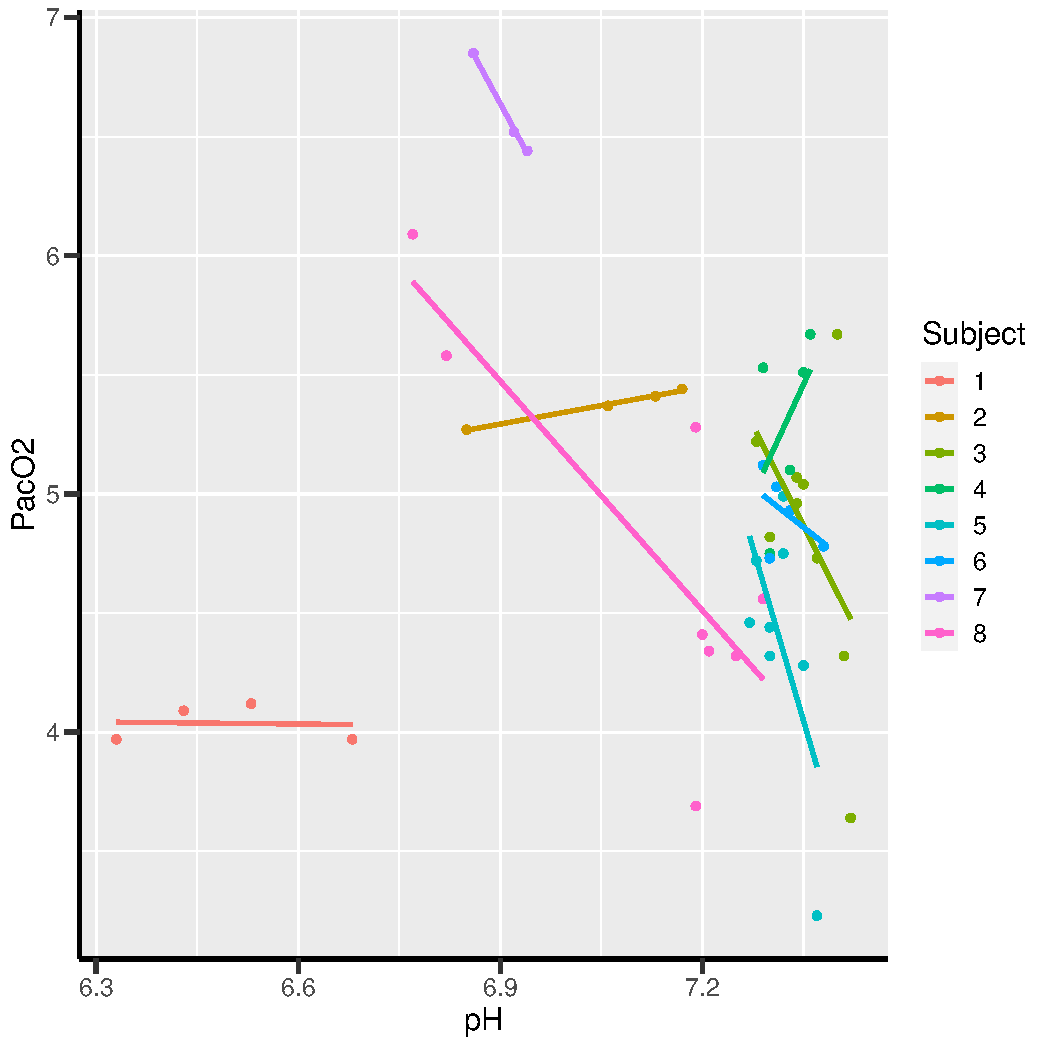
\includegraphics[trim={0 0 0 0},width=1\textwidth]{./figures/gg-describe-dataset.pdf}
\end{center}


\clearpage

\section{Partial partial in multiple linear regression}
\label{sec:org235ae36}

Consider the linear model:
\lstset{language=r,label= ,caption= ,captionpos=b,numbers=none}
\begin{lstlisting}
e.lmm <- lmm(pH ~ Subject + PacO2, data = bland1995)
eTable.lmm <- model.tables(e.lmm)
eTable.lmm
\end{lstlisting}

\begin{verbatim}
              estimate         se      df      lower       upper      p.value
(Intercept)  6.9298543 0.12946898 38.0076  6.6677598  7.19194884 0.000000e+00
Subject2     0.7046113 0.07735488 38.0076  0.5480155  0.86120702 4.269674e-11
Subject3     0.9500127 0.06109545 38.0076  0.8263322  1.07369313 0.000000e+00
Subject4     0.9715577 0.07350906 38.0076  0.8227474  1.12036807 8.881784e-16
Subject5     0.8603817 0.05839543 38.0076  0.7421671  0.97859630 0.000000e+00
Subject6     0.9264284 0.06599450 38.0076  0.7928304  1.06002642 0.000000e+00
Subject7     0.6921056 0.10490935 38.0076  0.4797291  0.90448203 8.662210e-08
Subject8     0.7033361 0.06157141 38.0076  0.5786921  0.82798005 7.438494e-14
PacO2       -0.1083230 0.02989281 38.0076 -0.1688375 -0.04780862 8.469583e-04
\end{verbatim}

We claim the partial correlation (adjusting \texttt{pH} and \texttt{PacO2} for
\texttt{Subject}) can be deduced from the Wald statistic and degrees of
freedom:

\begin{align}
\rho = \frac{\frac{\beta}{\sigma_{\beta}}}{\sqrt{\frac{\beta^2}{\sigma^2_{\beta}}+df}} = \frac{\beta}{\sqrt{\beta^2+df*\sigma_{\beta}^2}} \label{eq:pCor-formula}
\end{align}

\lstset{language=r,label= ,caption= ,captionpos=b,numbers=none}
\begin{lstlisting}
Wald <- eTable.lmm["PacO2","estimate"]/eTable.lmm["PacO2","se"]
Wald/sqrt(Wald^2+eTable.lmm["PacO2","df"])
\end{lstlisting}

\begin{verbatim}
[1] -0.5067321
\end{verbatim}


The proof can be split in three steps:
\begin{description}
\item[{1.}] the F-statistic testing the effect of each factor equals the
Wald-statistic squared (divided by 1, the number of parameters)
\end{description}

\lstset{language=r,label= ,caption= ,captionpos=b,numbers=none}
\begin{lstlisting}
Wald^2
\end{lstlisting}

\begin{verbatim}
[1] 13.13132
\end{verbatim}


\lstset{language=r,label= ,caption= ,captionpos=b,numbers=none}
\begin{lstlisting}
anova(e.lmm)
\end{lstlisting}

\begin{verbatim}
	     Multivariate Wald test 

              F-statistic       df  p.value    
mean: Subject      48.247 (7,38.0)  < 2e-16 ***
    : PacO2        13.131 (1,38.0) 0.000847 ***
\end{verbatim}


\begin{description}
\item[{2.}] this F-statistic equals \(\frac{MSSR}{MSSE}\) where \(MSSR =
  SSR/1\) and \(MSSE = SSE/(n-p)\) with \(SSE\) and \(SSR\) being the
explained and residual sum of squares. We can check that this
extends to multiple regression using the usual anova table:
\end{description}
\lstset{language=r,label= ,caption= ,captionpos=b,numbers=none}
\begin{lstlisting}
anova(lm(pH ~ Subject + PacO2, data = bland1995))
\end{lstlisting}

\begin{verbatim}
Analysis of Variance Table

Response: pH
          Df  Sum Sq Mean Sq F value    Pr(>F)    
Subject    7 2.86484 0.40926  46.600 < 2.2e-16 ***
PacO2      1 0.11532 0.11532  13.131 0.0008471 ***
Residuals 38 0.33373 0.00878                      
---
Signif. codes:  0 '***' 0.001 '**' 0.01 '*' 0.05 '.' 0.1 ' ' 1
\end{verbatim}


which is to be compared to\footnote{\Warning Since \Rlogo output type 1 anova only the last and second to
last line are relevant. The first line (\texttt{Subject}) is for a model
without \texttt{PacO2} so it should be expected that the F-value does not
match with the one of \texttt{Subject} in a model with \texttt{PacO2}.}

\lstset{language=r,label= ,caption= ,captionpos=b,numbers=none}
\begin{lstlisting}
sigma2 <- as.double(sigma(e.lmm))
beta <- eTable.lmm["PacO2","estimate"]
sigma_beta <- eTable.lmm["PacO2","se"]
c(MSSE = sigma2, MSSR = sigma2 * beta^2 /sigma_beta^2)
\end{lstlisting}

\begin{verbatim}
       MSSE        MSSR 
0.008782435 0.115324959
\end{verbatim}


This result can be easily proved when considering a model with a single
regressor:
\[ Y = X\beta + \varepsilon\text{, } \varepsilon\sim\Gaus(0,\sigma^2)\]
where we would have centered the outcome \(Y\). Here we denote by
\(X\) the design matrix, \(n\) the number of observations and \(p=1\)
the number of coefficients, \(H = X (X\trans{X})^{-1} \trans{X}\) the
hat matrix and \(\widehat{\beta} = (X\trans{X})^{-1} \trans{X}Y\) the
OLS estimator of the regression coefficients.
\begin{align*}
\Var(Y) = Y\trans{Y} =& YH\trans{Y} + Y(1-H)\trans{Y} \\
SST =& SSR + SSE \\
    =& \hat{\beta} (X\trans{X}) \trans{\hat{\beta}} + Y (1-H) \trans{Y} \\
    =& \sigma^2 (\hat{\beta} \Sigma^{-1}_{\hat{\beta}} \trans{\hat{\beta}} + n-p) \\
\frac{MSSR}{MSSE} &= \frac{\hat{\beta}^2}{\Sigma_{\hat{\beta}}} = Wald^2
\end{align*}

\begin{description}
\item[{3.}] the \(R^2\) is defined as the proportion of variance explained, so
using the previous results we get:
\end{description}
\begin{align*}
R^2 =& \frac{SSR}{SSR + SSE} \\
    =& \frac{1}{1 + SSE/SSR} \\
    =& \frac{1}{1 + (n-p)/(\beta^2/\sigma^2_\beta)} \\
    = \frac{Wald^2}{Wald^2 + n-p}
\end{align*}

This formula matches exactly the partial correlation coefficient when
\textbf{both} outcome are adjusted for \texttt{Subject}:
\lstset{language=r,label= ,caption= ,captionpos=b,numbers=none}
\begin{lstlisting}
e.partialCor <- partialCor(list(pH ~ Subject, PacO2 ~ Subject),
			   data = bland1995)
print(e.partialCor, digit = 5)
\end{lstlisting}

\begin{verbatim}
              estimate      se     df    lower   upper   p.value
rho(pH,PacO2) -0.50677 0.12514 25.674 -0.71027 -0.2251 0.0017753
\end{verbatim}


Similar values can be obtained using dedicated packages, e.g.:
\lstset{language=r,label= ,caption= ,captionpos=b,numbers=none}
\begin{lstlisting}
library(rmcorr)
rmcorr(Subject, PacO2, pH, bland1995)$r
\end{lstlisting}

\begin{verbatim}
[1] -0.5067697
\end{verbatim}


\clearpage

\section{Partial correlation with repeated measurements}
\label{sec:org2328ed5}

\subsection{Marginal and conditional correlation}
\label{sec:org144b47e}
There are several references on the subject
\citep{bland1995calculating,Lipsitz2001partial,bakdash2017repeated,shan2020correlation}. We
will focus on the mixed model approach. The idea is to jointly model
the variance and covariance of all measurements under appropriate
constrains. For instance denoting one measurement \(X\) and the other
measurement \(Y\), both indexed by time \(t\), our target parameter
may be \(\rho = \mathbb{C}or(X(t),Y(t))\) (marginal) assumed independent of
\(t\) while \(X\) and \(Y\) may or may not be stationnary. Another
target parameter could be the correlation between a de-noised version
of \(X\) and \(Y\), where we have for instance removed
individual-specific variations (conditional).

\bigskip

To be more specific let's consider the following statistical model:
\begin{align*}
X_i(t) &= \mu_{X}(t) + u_i + \varepsilon_{X,i}(t) \\
Y_i(t) &= \mu_{Y}(t) + v_i + \varepsilon_{Y,i}(t) \\
\text{where } \begin{bmatrix}u \\ v \\ \varepsilon_X(t) \\ \varepsilon_Y(t) \end{bmatrix}
&= \Gaus\left(\begin{bmatrix}0 \\ 0 \\ 0 \\ 0 \end{bmatrix},
\begin{bmatrix}
\tau_u & \tau_{uv} & 0 & 0 \\ \tau_{uv} & \tau_v & 0 & 0 \\ 
 0 & 0 & \sigma_X & \sigma_{XY} \\ 0 & 0 & \sigma_{XY} & \sigma_X \\ 
\end{bmatrix} \right)
\end{align*}
It implies the following residual covariance matrix:
\begin{align*}
\Omega = \Var\begin{bmatrix}X(1) \\ X(2) \\ X(3) \\ Y(1) \\ Y(2) \\ Y(3) \end{bmatrix}
&= \begin{bmatrix}
\tau_u + \sigma_X & \tau_u & \tau_u & \tau_{uv} + \sigma_{XY} & \tau_{uv} & \tau_{uv} \\
\tau_u & \tau_u + \sigma_X & \tau_u & \tau_{uv} & \tau_{uv} + \sigma_{XY} & \tau_{uv} \\
\tau_u & \tau_u & \tau_u + \sigma_X & \tau_{uv} & \tau_{uv} & \tau_{uv} + \sigma_{XY} \\
\tau_{uv} + \sigma_{XY} & \tau_{uv}  & \tau_{uv} & \tau_v + \sigma_Y & \tau_v & \tau_v \\
\tau_{uv} & \tau_{uv} + \sigma_{XY} & \tau_{uv}  & \tau_v & \tau_v + \sigma_Y & \tau_v \\
\tau_{uv} & \tau_{uv} & \tau_{uv} + \sigma_{XY}  & \tau_v & \tau_v & \tau_v + \sigma_Y  \\
\end{bmatrix} \\
&= \begin{bmatrix}
\sigma_1 & \sigma_2 & \sigma_2 & \sigma_3 & \sigma_4 & \sigma_4 \\
\sigma_2 & \sigma_1 & \sigma_2 & \sigma_4 & \sigma_3 & \sigma_4 \\
\sigma_2 & \sigma_2 & \sigma_1 & \sigma_4 & \sigma_4 & \sigma_3 \\
\sigma_3 & \sigma_4 & \sigma_4 & \sigma_5 & \sigma_6 & \sigma_6 \\
\sigma_4 & \sigma_3 & \sigma_4 & \sigma_6 & \sigma_5 & \sigma_6 \\
\sigma_4 & \sigma_4 & \sigma_3 & \sigma_6 & \sigma_6 & \sigma_5  \\
\end{bmatrix}
\end{align*}
and the following residual correlation matrix:
\[ R = \mathbb{C}or\begin{bmatrix}X(1) \\ X(2) \\ X(3) \\ Y(1) \\ Y(2) \\ Y(3) \end{bmatrix}
= \begin{bmatrix}
1      & \rho_1 & \rho_1 & \rho_2 & \rho_3 & \rho_3 \\
\rho_1 & 1      & \rho_1 & \rho_3 & \rho_2 & \rho_3 \\
\rho_1 & \rho_1 & 1      & \rho_3 & \rho_3 & \rho_2 \\
\rho_2 & \rho_3 & \rho_3 & 1      & \rho_4 & \rho_4 \\
\rho_3 & \rho_2 & \rho_3 & \rho_4 & 1      & \rho_4 \\
\rho_3 & \rho_3 & \rho_2 & \rho_4 & \rho_4 & 1  \\
\end{bmatrix}
\]


The marginal correlation is:
\begin{align*}
\rho_M &= \frac{\Cov[u_i + \varepsilon_{X,i}(t),v_i + \varepsilon_{Y,i}(t)]}{\sqrt{\Var[u_i + \varepsilon_{X,i}(t)]\Var[v_i + \varepsilon_{Y,i}(t)]}} \\
&= \frac{\tau_{uv} + \sigma_{XY}}{\sqrt{(\tau_u+\sigma_X)(\tau_v+\sigma_Y)}} = \frac{\sigma_3}{\sqrt{\sigma_1\sigma_5}} =  \rho_2
\end{align*}
while the conditional correlation is:
\begin{align*}
\rho_C &= \frac{\Cov[\varepsilon_{X,i}(t),\varepsilon_{Y,i}(t)]}{\sqrt{\Var[\varepsilon_{X,i}(t)]\Var[\varepsilon_{Y,i}(t)]}} \\
&= \frac{\sigma_{XY}}{\sqrt{\sigma_X\sigma_Y}} = \frac{\sigma_3-\sigma_4}{\sqrt{(\sigma_1-\sigma_2)(\sigma_5-\sigma_6)}} =  \frac{\rho_2-\rho_3}{\sqrt{(1-\rho_1)(1-\rho_2)}}
\end{align*}

\subsection{Approximated conditional correlation}
\label{sec:org4b5632d}

We now show that formula \ref{eq:pCor-formula} generalizes to mixed
models. Consider the following mixed model relating \(\VY =
(Y_1,\ldots,Y_T)\) and \(\VX = (X_1,\ldots,X_T)\):
\[ \VY = \VX \beta + \Vvarepsilon \]
where \(\boldsymbol{\varepsilon}\sim\Gaus[0,\Omega]\). Introducing the
cholesky decomposition \(\Omega = \omega\trans{\omega}\), we can equivalently study:
\[ \omega^{-1}\VY = \omega^{-1}\VX + \boldsymbol{\zeta} \]
where \(\boldsymbol{\zeta}\) follow a standard normal distribution. We
are back the univariate case up to a factor \(\omega^{-1}\).

\begin{description}
\item[{1.}] F-statistics are still equal the Wald statistic squared
(divided by the number of parameters).
\item[{2.}] F-statistics still equal \(\frac{MSSR}{MSSE}\). Indeed:
\end{description}
\begin{align*}
SSE &= \trans{\left(\omega^{-1}\VY\right)}\left(I-\omega^{-1}\VX\left(\trans{\left(\omega^{-1}\VX\right)}\left(\omega^{-1}\VX\right)\right)^{-1} \trans{\left(\omega^{-1}\VX\right)}\right)\left(\omega^{-1}\VY\right) \\
&= \trans{\VY} \Omega^{-1} \VY - \trans{\VY} \Omega^{-1} \VX \left(\trans{\VX}\Omega^{-1}\VX\right)^{-1} \trans{\VX} \Omega^{-1} \VY  \\
&= \trans{\VY} (I-\trans{H})\Omega^{-1} (I-\trans{H}) \VY
\end{align*}
where \(H = \VX \left(\trans{\VX}\Omega^{-1} \VX \right)^{-1}
\trans{\VX} \Omega^{-1}\). Indeed:
\[ (I-\trans{H})\Omega^{-1}
(I-\trans{H})= \Omega^{-1} - \trans{H}\Omega^{-1} - \Omega^{-1} H +
\trans{H}\Omega^{-1}H = \Omega^{-1} - \trans{H}\Omega^{-1} \]
and \(MSSE = \frac{SSE}{n-p} = \sigma^2\) with \(p\) being the rank
of \(X\). Using that \(HH=H\) :
\begin{align*}
SSR &= \trans{\left(\omega^{-1}\VY\right)}\left(\omega^{-1}\VX\left(\trans{\left(\omega^{-1}\VX\right)}\left(\omega^{-1}\VX\right)\right)^{-1} \trans{\left(\omega^{-1}\VX\right)}\right)\left(\omega^{-1}\VY\right) \\
&= \trans{\VY} \Omega^{-1} \VX \left(\trans{\VX}\Omega^{-1}\VX\right)^{-1} \trans{\VX} \Omega^{-1} \VY  \\
&= \trans{\VY} \trans{H} \Omega^{-1} \VY = \trans{\VY} \trans{H}\trans{H} \Omega^{-1} \VY  \\
&= \trans{\VY} \trans{H} \Omega^{-1} H \VY \\
&= \trans{\widehat{\beta}} \trans{X} \Omega^{-1} X \widehat{\beta}  = \trans{\widehat{\beta}} \Sigma^{-1}_{\widehat{\beta}} \widehat{\beta} 
\end{align*}
where \(\widehat{\beta} = \left(\trans{\VX}\Omega^{-1} \VX
\right)^{-1}\trans{\VX} \Omega^{-1}\VY\) is the GLS estimator of
\(\beta\). So for a single covariate: 
\[ F=\frac{MSSR}{MSSE}=\frac{\widehat{\beta}\Sigma^{-1}\widehat{\beta}}{\sigma^2} \]

\begin{description}
\item[{3.}] Defining \(R^2\) as the proportion of variance explained, we get back
\end{description}
\[ R^2 = \frac{\beta^2}{\beta^2 + df \sigma^2_{\beta} } \]
where \(df=n-p\). A corresponding correlation coefficient can computed as:
\[ \rho = \frac{\beta}{\sqrt{\beta^2 + df \sigma^2_{\beta}} } \]

\clearpage

\subsection{Back to the example}
\label{sec:org4cb0eea}

In the example, we see a very small marginal correlation and a large conditional one:
\lstset{language=r,label= ,caption= ,captionpos=b,numbers=none}
\begin{lstlisting}
e.pcor <- partialCor(c(pH,PacO2)~1, repetition = ~time|Subject, data = bland1995, heterogeneous = 0.5)
e.pcor
\end{lstlisting}

\begin{verbatim}
                   estimate    se   df  lower    upper p.value
rho(1.pH,1.PacO2) -1.63e-05 0.313 1.23 -0.989 0.988993  1.0000
r(1.pH,1.PacO2)   -5.09e-01 0.125 2.59 -0.808 0.000496  0.0501
\end{verbatim}


This matches the estimate (but not the uncertainty) of another software:
\lstset{language=r,label= ,caption= ,captionpos=b,numbers=none}
\begin{lstlisting}
c(r = rmcorr(Subject, pH, PacO2, bland1995)$r,
  p = rmcorr(Subject, pH, PacO2, bland1995)$p)
\end{lstlisting}

\begin{verbatim}
            r             p 
-0.5067697422  0.0008471081
\end{verbatim}


We can also extract the underlying correlation coefficients:
\lstset{language=r,label= ,caption= ,captionpos=b,numbers=none}
\begin{lstlisting}
round(coef(attr(e.pcor,"lmm"), effects = "correlation"),5)
\end{lstlisting}

\begin{verbatim}
rho(1.pH,1.PacO2)    rho(1.pH,2.PacO2) rho(1.PacO2,2.PacO2) 
         -0.00002              0.10168              0.66317 
   rho(1.pH,2.pH) 
          0.88129
\end{verbatim}


that reveal a very strong within \texttt{pH} correlation (almost 0.9) and a
rather strong within \texttt{PacO2} correlation (about 0.65). The
instantaneous correlation is nearly 0 but the lag correlation is about
0.1 leading to the observed conditional correlation.

\bigskip

An alternative approach is to fit a mixed model on only one outcome,
regressing out the other:
\lstset{language=r,label= ,caption= ,captionpos=b,numbers=none}
\begin{lstlisting}
e.CS <- lmm(pH ~ PacO2, repetition = ~time|Subject, data = bland1995,
	    structure = "CS")
\end{lstlisting}

Then estimate the partial correlation formula:
\lstset{language=r,label= ,caption= ,captionpos=b,numbers=none}
\begin{lstlisting}
e.CSaov <- anova(e.CS, effects = "PacO2=0")
confint(e.CSaov, columns = c("estimate","se","df","partial.r"))
\end{lstlisting}

\begin{verbatim}
      estimate     se   df partial.r
PacO2   -0.103 0.0295 39.6    -0.486
\end{verbatim}


\clearpage

Here approximate degrees of freedom are used, i.e. 39.6 instead of:
\lstset{language=r,label= ,caption= ,captionpos=b,numbers=none}
\begin{lstlisting}
NROW(bland1995)-2
\end{lstlisting}

\begin{verbatim}
[1] 45
\end{verbatim}


which would lead to a correlation of:
\lstset{language=r,label= ,caption= ,captionpos=b,numbers=none}
\begin{lstlisting}
e.CSaov$univariate$statistic/sqrt(e.CSaov$univariate$statistic^2+45)
\end{lstlisting}

\begin{verbatim}
[1] -0.4627676
\end{verbatim}


Finally we could also compute the Person's correlation (ignoring
repeated measurements):
\lstset{language=r,label= ,caption= ,captionpos=b,numbers=none}
\begin{lstlisting}
cor(dtW$pH,dtW$PacO2)
\end{lstlisting}

\begin{verbatim}
[1] -0.06521774
\end{verbatim}


and use a bootstrap at the individual level for assessing the
uncertainty:
\lstset{language=r,label= ,caption= ,captionpos=b,numbers=none}
\begin{lstlisting}
library(boot)
library(data.table)
dtW <- as.data.table(bland1995)
dtL <- dcast(dtW, value.var = c("pH","PacO2"), formula = Subject ~ time)
calcCor <- function(data, statistic){
  data2 <- data[statistic]
  data3 <- melt(data2, id.vars = c("Subject"), 
		measure=patterns("pH","PacO2"),
		variable.name = "time", value.name = c("pH","PacO2"))
  cor(data3$pH, data3$PacO2)
}
e.boot <- boot(dtW, calcCor, R = 1000)
e.boot
\end{lstlisting}

\begin{verbatim}

ORDINARY NONPARAMETRIC BOOTSTRAP


Call:
boot(data = dtW, statistic = calcCor, R = 1000)


Bootstrap Statistics :
       original      bias    std. error
t1* -0.06521774 -0.01635557   0.1989813
\end{verbatim}

In summary we have obtained the following estimates:
\begin{itemize}
\item for the marginal correlation
\end{itemize}
\lstset{language=r,label= ,caption= ,captionpos=b,numbers=none}
\begin{lstlisting}
out.naive <- c(estimate = e.boot$t0, se = sd(e.boot$t), df = NA,
	       lower = boot.ci(e.boot, type = "perc")$percent[4],
	       upper = boot.ci(e.boot, type = "perc")$percent[5],
	       p.value = NA)
e.pcor2 <- partialCor(c(pH,PacO2)~1, repetition = ~time|Subject, df = FALSE,
		      data = bland1995, heterogeneous = 0.5)
\end{lstlisting}

\begin{itemize}
\item for the conditional correlation
\end{itemize}
\lstset{language=r,label= ,caption= ,captionpos=b,numbers=none}
\begin{lstlisting}
e.rmcorr <- rmcorr(Subject, PacO2, pH, bland1995)
out.rmcorr <- c(estimate = e.rmcorr$r, se = NA, df = e.rmcorr$df,
		lower = e.rmcorr[[4]][1], upper = e.rmcorr[[4]][2], p.value = e.rmcorr[[3]])
out.magic <- estimate(e.CS, f = function(p){
  e.vcov <- vcov(e.CS, df = TRUE, p = p)
  p["PacO2"]/sqrt(p["PacO2"]^2+e.vcov["PacO2","PacO2"]*attr(e.vcov,"df")["PacO2"])
})
\end{lstlisting}

So overall:
\lstset{language=r,label= ,caption= ,captionpos=b,numbers=none}
\begin{lstlisting}
out <- rbind(
  data.frame(type = "marginal", rbind(naive = out.naive, lmmM = e.pcor2[1,])),
  data.frame(type = "conditional", rbind(rmcorr = out.rmcorr, lmmC = e.pcor2[2,], magic = out.magic))
)
out <- cbind(name = rownames(out), out)
rownames(out) <- NULL
out
\end{lstlisting}

\begin{verbatim}
    name        type      estimate         se       df      lower      upper      p.value
1  naive    marginal -6.521774e-02 0.19898132       NA -0.5183738  0.2809898           NA
2   lmmM    marginal -1.627833e-05 0.31296494      Inf -0.5465274  0.5465046 9.999585e-01
3 rmcorr conditional -5.067697e-01         NA 38.00000 -0.7112297 -0.2232550 8.471081e-04
4   lmmC conditional -5.085547e-01 0.12542915      Inf -0.7043437 -0.2408608 4.862469e-04
5  magic conditional -4.864796e-01 0.08698358 30.83874 -0.6639214 -0.3090378 3.992869e-06
\end{verbatim}


\lstset{language=r,label= ,caption= ,captionpos=b,numbers=none}
\begin{lstlisting}
gg.forest <- ggplot(out, aes(x = name, y = estimate, color = type))
gg.forest <- gg.forest + geom_hline(yintercept=0, linetype = 2)
gg.forest <- gg.forest + geom_point(size = 2) + geom_errorbar(aes(ymin = lower, ymax = upper))
gg.forest <- gg.forest + coord_flip() 
gg.forest
\end{lstlisting}

\subsection{Simulation study (compound symmetry model)}
\label{sec:org6ca2fe1}

We'll compare \(\rho\) and \(r\) in the case of 3 timepoints,
\(r=0.8\), and 250 individuals:
\lstset{language=r,label= ,caption= ,captionpos=b,numbers=none}
\begin{lstlisting}
n.time <- 3
n.id <- 250
Sigma <- matrix(c(1,0.8,0.8,1),2,2)
Sigma
\end{lstlisting}

\begin{verbatim}
     [,1] [,2]
[1,]  1.0  0.8
[2,]  0.8  1.0
\end{verbatim}


\lstset{language=r,label= ,caption= ,captionpos=b,numbers=none}
\begin{lstlisting}
set.seed(11)
df.W <- data.frame(id = unlist(lapply(1:n.id, rep, n.time)),
		   time = rep(1:n.time,n.id),
		   rmvnorm(n.time*n.id, mean = c(3,3), sigma = Sigma)
		   )
head(df.W)
\end{lstlisting}

\begin{verbatim}
  id time       X1       X2
1  1    1 2.483259 2.759470
2  1    2 1.034157 1.102983
3  1    3 3.636308 2.691506
4  2    1 4.463341 4.150878
5  2    2 2.510048 2.081439
6  2    3 2.103239 2.317938
\end{verbatim}


\clearpage

We use random effects to obtain a constant correlation within \(X\)
and within \(Y\):
\lstset{language=r,label= ,caption= ,captionpos=b,numbers=none}
\begin{lstlisting}
sd.id <- 1.5
df.W$X1 <- df.W$X1 + rnorm(n.id, sd = sd.id/4)[df.W$id]
df.W$X2 <- df.W$X2 + rnorm(n.id, sd = sd.id)[df.W$id]
df.W$id <- as.factor(df.W$id)
df.L <- reshape2::melt(df.W, id.vars = c("id","time")) 
df.L$time2 <- as.factor(as.numeric(as.factor(paste(df.L$variable,df.L$time,sep="."))))
\end{lstlisting}

This will lead to the following correlation structure:
\lstset{language=r,label= ,caption= ,captionpos=b,numbers=none}
\begin{lstlisting}
Sigma.GS <- as.matrix(bdiag(Sigma,Sigma,Sigma))[c(1,3,5,2,4,6),c(1,3,5,2,4,6)]
Sigma.GS[1:3,1:3] <- Sigma.GS[1:3,1:3] + (sd.id/4)^2
Sigma.GS[4:6,4:6] <- Sigma.GS[4:6,4:6] + sd.id^2
cov2cor(Sigma.GS)
\end{lstlisting}

\begin{verbatim}
          [,1]      [,2]      [,3]      [,4]      [,5]      [,6]
[1,] 1.0000000 0.1232877 0.1232877 0.4155056 0.0000000 0.0000000
[2,] 0.1232877 1.0000000 0.1232877 0.0000000 0.4155056 0.0000000
[3,] 0.1232877 0.1232877 1.0000000 0.0000000 0.0000000 0.4155056
[4,] 0.4155056 0.0000000 0.0000000 1.0000000 0.6923077 0.6923077
[5,] 0.0000000 0.4155056 0.0000000 0.6923077 1.0000000 0.6923077
[6,] 0.0000000 0.0000000 0.4155056 0.6923077 0.6923077 1.0000000
\end{verbatim}


We can now estimate two types of correlation: marginal and conditional
\lstset{language=r,label= ,caption= ,captionpos=b,numbers=none}
\begin{lstlisting}
e.LMMstar <- partialCor(c(X1,X2) ~ 1, repetition = ~ time|id, data = df.W, heterogeneous = 0.5)
e.LMMstar
\end{lstlisting}

\begin{verbatim}
		Partial correlation 

               estimate     se   df lower upper  p.value
rho(1.X1,1.X2)    0.427 0.0346 34.7 0.356 0.493 6.76e-13
r(1.X1,1.X2)      0.798 0.0251 58.9 0.764 0.829 0.00e+00
	----------------------------------------------------
	rho: marginal correlation 
	r  : correlation conditional on the individual 
	estimates, standard errors, confidence intervals have been back-transformed (tanh).
\end{verbatim}


The conditional coefficient is identical to what other packages output:
\lstset{language=r,label= ,caption= ,captionpos=b,numbers=none}
\begin{lstlisting}
rmcorr:::rmcorr(id, X1, X2, df.W)$r
\end{lstlisting}

\begin{verbatim}
[1] 0.7983617
\end{verbatim}


Here the modeled correlation matrix is:
\lstset{language=r,label= ,caption= ,captionpos=b,numbers=none}
\begin{lstlisting}
Omega <- sigma(attr(e.LMMstar,"lmm"))
Rho <- cov2cor(Omega)
Rho
\end{lstlisting}

\begin{verbatim}
            1.X1        2.X1        3.X1        1.X2        2.X2        3.X2
1.X1  1.00000000  0.06545230  0.06545230  0.42652595 -0.00432106 -0.00432106
2.X1  0.06545230  1.00000000  0.06545230 -0.00432106  0.42652595 -0.00432106
3.X1  0.06545230  0.06545230  1.00000000 -0.00432106 -0.00432106  0.42652595
1.X2  0.42652595 -0.00432106 -0.00432106  1.00000000  0.68836567  0.68836567
2.X2 -0.00432106  0.42652595 -0.00432106  0.68836567  1.00000000  0.68836567
3.X2 -0.00432106 -0.00432106  0.42652595  0.68836567  0.68836567  1.00000000
\end{verbatim}


From which the conditional correlation can be deduced:
\lstset{language=r,label= ,caption= ,captionpos=b,numbers=none}
\begin{lstlisting}
(Rho[1,4]-Rho[1,5])/sqrt((1-Rho[1,2])*(1-Rho[4,5]))
\end{lstlisting}

\begin{verbatim}
[1] 0.7983617
\end{verbatim}


or equivalently:
\lstset{language=r,label= ,caption= ,captionpos=b,numbers=none}
\begin{lstlisting}
(Omega[1,4]-Omega[1,5])/sqrt((Omega[1,1]-Omega[1,2])*(Omega[4,4]-Omega[4,5]))
\end{lstlisting}

\begin{verbatim}
[1] 0.7983617
\end{verbatim}


Replicating this a thousand times:
\lstset{language=r,label= ,caption= ,captionpos=b,numbers=none}
\begin{lstlisting}
n.id <- 100
n.sim <- 1000
n.cpus <- 25 ## run on the server
warper <- function(n){ 
  df.W <- data.frame(id = unlist(lapply(1:n, rep, n.time)),
		     time = rep(1:n.time,n),
		     rmvnorm(n.time*n, mean = c(3,3), sigma = Sigma)
		     )
  df.W$X1 <- df.W$X1 + rnorm(n, sd = sd.id/4)[df.W$id]
  df.W$X2 <- df.W$X2 + rnorm(n, sd = sd.id)[df.W$id]
  df.W$id <- as.factor(df.W$id)

  res1 <- setNames(c(rmcorr(id, X1, X2, df.W)$r, rmcorr(id, X1, X2, df.W)$CI), c("estimate","lower","upper"))
  res2 <- partialCor(c(X1,X2) ~ 1, repetition = ~ time|id, data = df.W, heterogeneous = 0.5)
  return(rbind(cbind(as.data.frame(as.list(res1)), se = NA, method = "rmcorr"),
	       cbind(res2[2,c("estimate","lower","upper","se")],method="lmm")))
}

ls.res <- pbapply::pblapply(1:n.sim,function(iSim){
  cbind(sim = iSim, warper(n.id))
}, cl = n.cpus)
dt.res <- as.data.table(do.call(rbind, ls.res))
\end{lstlisting}

lead to the same estimate for the two implementations:
\lstset{language=r,label= ,caption= ,captionpos=b,numbers=none}
\begin{lstlisting}
range(dt.res[method=="rmcorr",estimate]-dt.res[method=="lmm",estimate], na.rm=TRUE)
\end{lstlisting}

\begin{verbatim}
[1] -8.572216e-10  2.108167e-09
\end{verbatim}


and lead to a reasonnable coverage:
\lstset{language=r,label= ,caption= ,captionpos=b,numbers=none}
\begin{lstlisting}
dt.res[,.(missing = mean(is.na(estimate)), coverage = mean((0.8>=lower)*(0.8<=upper), na.rm=TRUE)), by = "method"]
\end{lstlisting}

\begin{verbatim}
   method missing coverage
1: rmcorr   0.000 0.941000
2:    lmm   0.026 0.949692
\end{verbatim}

\subsection{Simulation study (crossed random effect model)}
\label{sec:org9bb6802}

We will modify the previous simulation setting by introducing more
structure on the correlation. More precisely, observations will be
correlated within individual (biological variation) and within
timepoint (batch effect). This violates the compound symmetry
structure and therefore we expect \texttt{rmcorr} to give biased
estimates. We will use \texttt{lmer} instead of \texttt{lmm} as a reference since
\texttt{lmer} is very convenient to use and fast when dealing with crossed
random effects. Note that, however, it is not straightforward to have a
measure of uncertainty.

\lstset{language=r,label= ,caption= ,captionpos=b,numbers=none}
\begin{lstlisting}
n.time <- 4
n.id <- 100
warper <- function(n){
  df.W <- data.frame(id = unlist(lapply(1:n.id, rep, n.time)),
		     time = rep(1:n.time,n.id),
		     rmvnorm(n.time*n.id, mean = c(3,3), sigma = Sigma)
		     )
  df.W$X1 <- df.W$X1 + rnorm(n.id, sd = sd.id/4)[df.W$id]
  df.W$X2 <- df.W$X2 + rnorm(n.id, sd = sd.id)[df.W$id]
  df.W$X1 <- df.W$X1 + rnorm(n.time, sd = sd.id/3)[df.W$time]
  df.W$X2 <- df.W$X2 + rnorm(n.time, sd = sd.id/2)[df.W$time]
  df.W$id <- as.factor(df.W$id)
  df.W$time <- as.factor(df.W$time)

  e.lm <- lm(X1~X2+id+time, data = df.W)
  e.Slm <- summary(e.lm)$coef

  e.lmer <- lmer(X2 ~ X1 + (1|time) + (1|id), data = df.W)
  e.Slmer <- summary(e.lmer)$coefficient

  res0 <- c(estimate = e.Slm["X2","t value"]/sqrt(e.Slm["X2","t value"]^2+df.residual(e.lm)), lower = NA, upper = NA)
  res1 <- setNames(c(rmcorr(id, X1, X2, df.W)$r, rmcorr(id, X1, X2, df.W)$CI), c("estimate","lower","upper"))
  res2 <- c(estimate = e.Slmer["X1","t value"]/sqrt(e.Slmer["X1","t value"]^2+e.Slmer["X1","df"]), lower = NA, upper = NA)

  return(rbind(cbind(as.data.frame(as.list(res0)), method = "lm"),
	       cbind(as.data.frame(as.list(res1)), method = "rmcorr"),
	       cbind(as.data.frame(as.list(res2)), method= "lmer")))
}

ls.res <- pbapply::pblapply(1:101,function(iSim){
  cbind(sim = iSim, warper(100))
})
dt.res <- as.data.table(do.call(rbind, ls.res))
\end{lstlisting}

We can clearly see that the \texttt{rmcorr} estimator is biased and very
variable while the \texttt{lmer}-based estimator (i.e. using
\autoref{eq:pCor-formula}) gives reasonnable results:
\lstset{language=r,label= ,caption= ,captionpos=b,numbers=none}
\begin{lstlisting}
rbind(lm = quantile(dt.res[method=="lm",estimate]),
      rmcorr = quantile(dt.res[method=="rmcorr",estimate]),
      lmer = quantile(dt.res[method=="lmer",estimate]))
\end{lstlisting}

\begin{verbatim}
               0%       25%       50%       75%      100%
lm     0.74113022 0.7802503 0.7989544 0.8145657 0.8544672
rmcorr 0.05260171 0.4773873 0.6189341 0.7273679 0.8425171
lmer   0.73416614 0.7739002 0.7937885 0.8103669 0.8529145
\end{verbatim}


Note that the linear regression approach can be fixed in that example
by adjusting on time. However with more complex covariance pattern it
may not always be possible to find an appropriate \texttt{lm} approach.

\section{Reference}
\label{sec:orgba0cd87}
\begingroup
\renewcommand{\section}[2]{}
\bibliographystyle{apalike}
\bibliography{bibliography} 
\endgroup

\appendix \titleformat{\section}
{\normalfont\Large\bfseries}{}{1em}{Appendix~\thesection:~}

\renewcommand{\thefigure}{\Alph{figure}}
\renewcommand{\thetable}{\Alph{table}}
\renewcommand{\theequation}{\Alph{equation}}

\setcounter{figure}{0}    
\setcounter{table}{0}    
\setcounter{equation}{0}    
\end{document}